\chapter{Computer Architecture}

\section{Introduction to Computer Architecture}
Computer architecture refers to the design and organization of a
computer's components. Every computer from past to present, have a
structure divided into five categories. Five classic components of a
computer are —

\begin{minipage}[TH]{0.76\textwidth}
   \begin{itemize}
      \item \textbf{Control Unit:} This component manages the operations of the computer. It directs the flow of data between the CPU and other components.
      \item \textbf{Memory:} This is where data and instructions are stored. It is a crucial part of the computer system that allows for the storage and retrieval of information.
      \item \textbf{Datapath:} The component of the processor that performs arithmetic operations e.g ALU, Registers and Bus.
      \item \textbf{Input:} This refers to the devices or methods through which data is entered into the computer system.
      \item \textbf{Output:} This refers to the devices or methods through which data is presented to the user or other systems.
   \end{itemize}
\end{minipage}\hfill
\begin{minipage}[TH]{0.22\textwidth}
   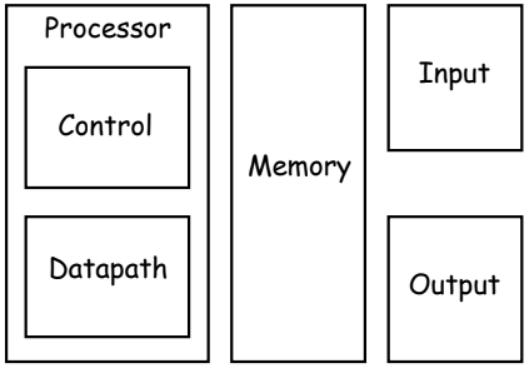
\includegraphics[width=\linewidth]{figures/computer_architecture.png}
\end{minipage}

% \subsection{Von Neumann architecture}
% \begin{center}
%    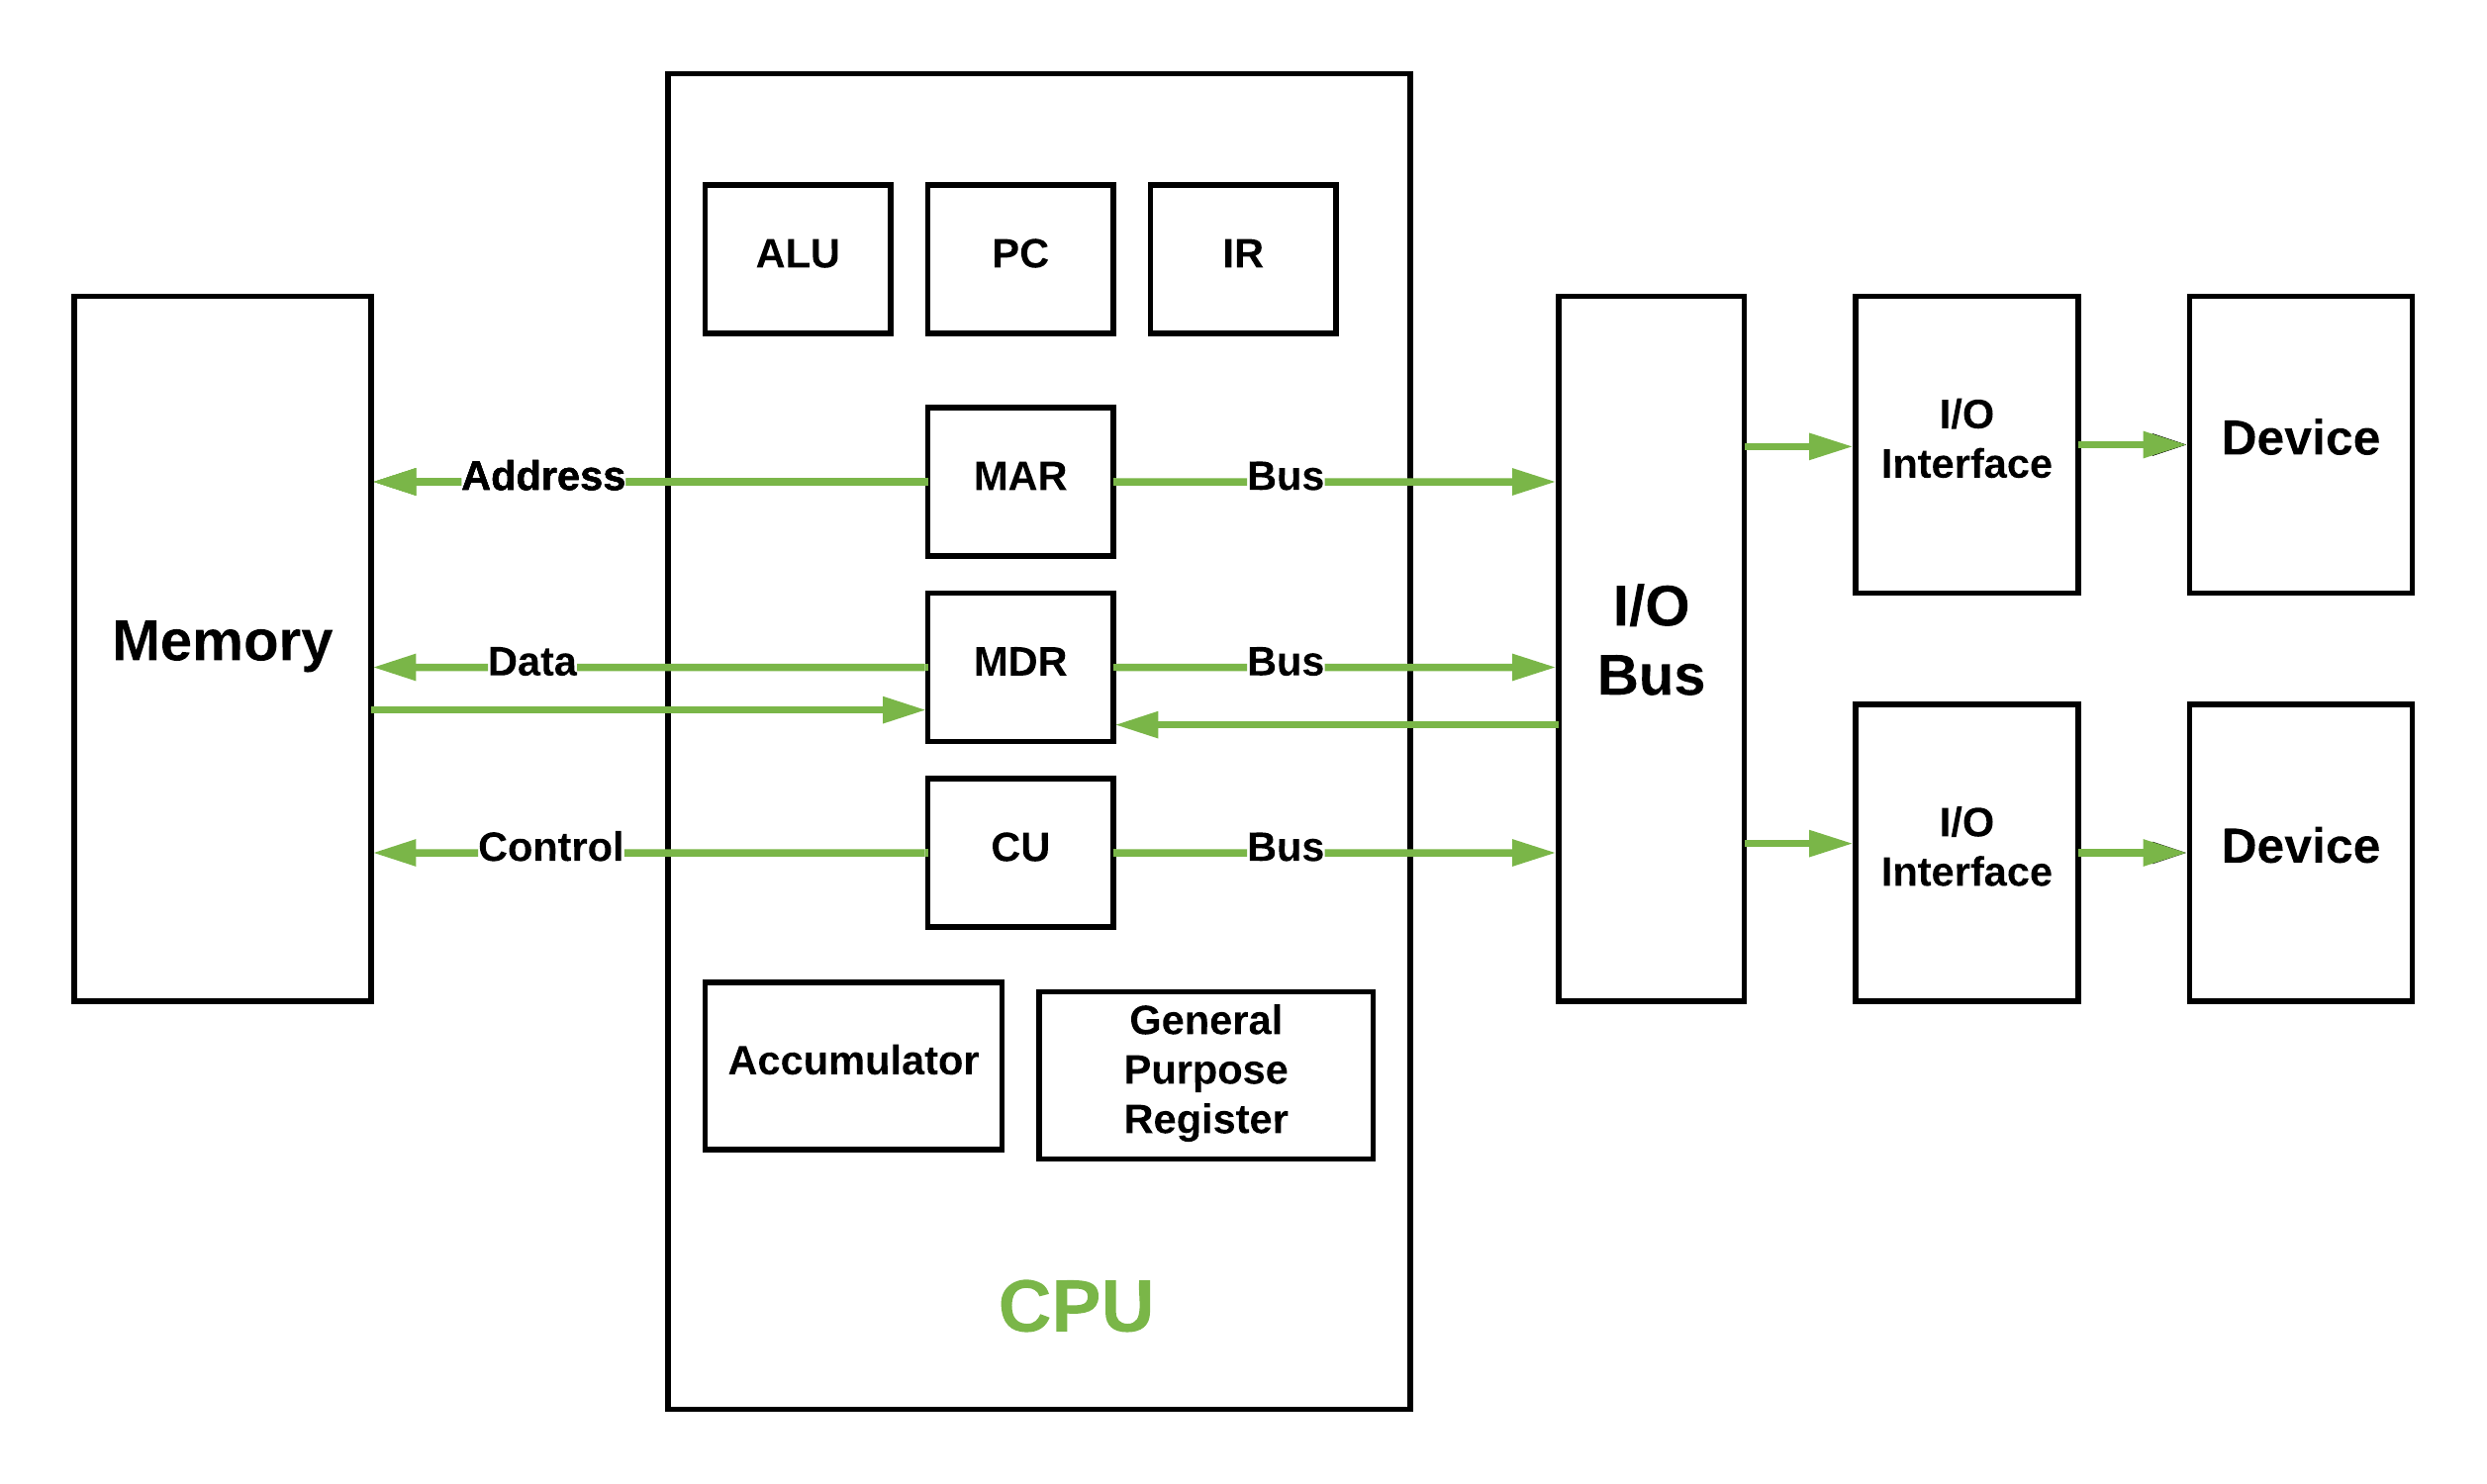
\includegraphics[width=0.58\linewidth]{figures/Von-Neumann.png}
% \end{center}

% The two key principles of the Von Neumann architecture are:
% \begin{enumerate}[left=0pt]
%    \item \textbf{Stored Program Concept:} Both data and instructions are stored in the same memory, allowing the computer to be programmable and flexible. Also address and data bus shared. 
%    \item \textbf{Sequential Instruction Execution:} Instructions are fetched and executed one at a time in a specific order, simplifying processing and control.
% \end{enumerate}


\subsection{The Role of Buses}
\begin{itemize}[parsep=0.4em]
   \item \textbf{\textit{Data Bus}:} Transfers data between components.
   \item \textbf{\textit{Address Bus}:} Carries the memory addresses for data retrieval.
   \item \textbf{\textit{Control Bus}:} Sends control signals to manage the flow of data and instructions.
\end{itemize}

\subsection{Types of Processor}
\begin{itemize}[parsep=0.4em]
   \item \textbf{\textit{CISC (Complex Instruction Set Computer)}:}\\
   A processor that uses complex instructions with many addressing modes.
   \item \textbf{\textit{RISC (Reduced Instruction Set Computer)}:}\\
   A processor with a small, simple set of instructions, making it faster for many tasks.
   \item \textbf{\textit{DSP (Digital Signal Processor)}:}\\
   A specialized processor used for handling signal processing, often used in audio or video applications.
\end{itemize}

\subsection{Types of Memory}
\begin{itemize}[parsep=0.25em]
   \item Registers: Fastest, but smallest form of memory.
   \item Cache: Stores frequently accessed data for quicker access.
   \item Main Memory (RAM): Primary memory for active tasks.
   \item Secondary Storage (Hard Disk, SSD): Long-term storage for data.
\end{itemize}


\subsection{Layers of Computer}
\begin{minipage}{0.75\textwidth}
   $\bullet$ \ \
   \textbf{Hardware:} Physical components of the computer.\\[0.5em]
   $\bullet$ \ \
   \textbf{Operating System:} Software that manages hardware and software resources.\\[0.5em]
   $\bullet$ \ \
   \textbf{Applications:} Programs that perform specific tasks for users.

   \vspace{1em}
   The layers of software may compose of Application Software and System Software. These can be organized primarily in a hierarchical fashion, with applications being the outermost ring and a variety of systems soft ware sitting between the hardware and applications software.
\end{minipage}\hfill
\begin{minipage}{0.2\textwidth}
   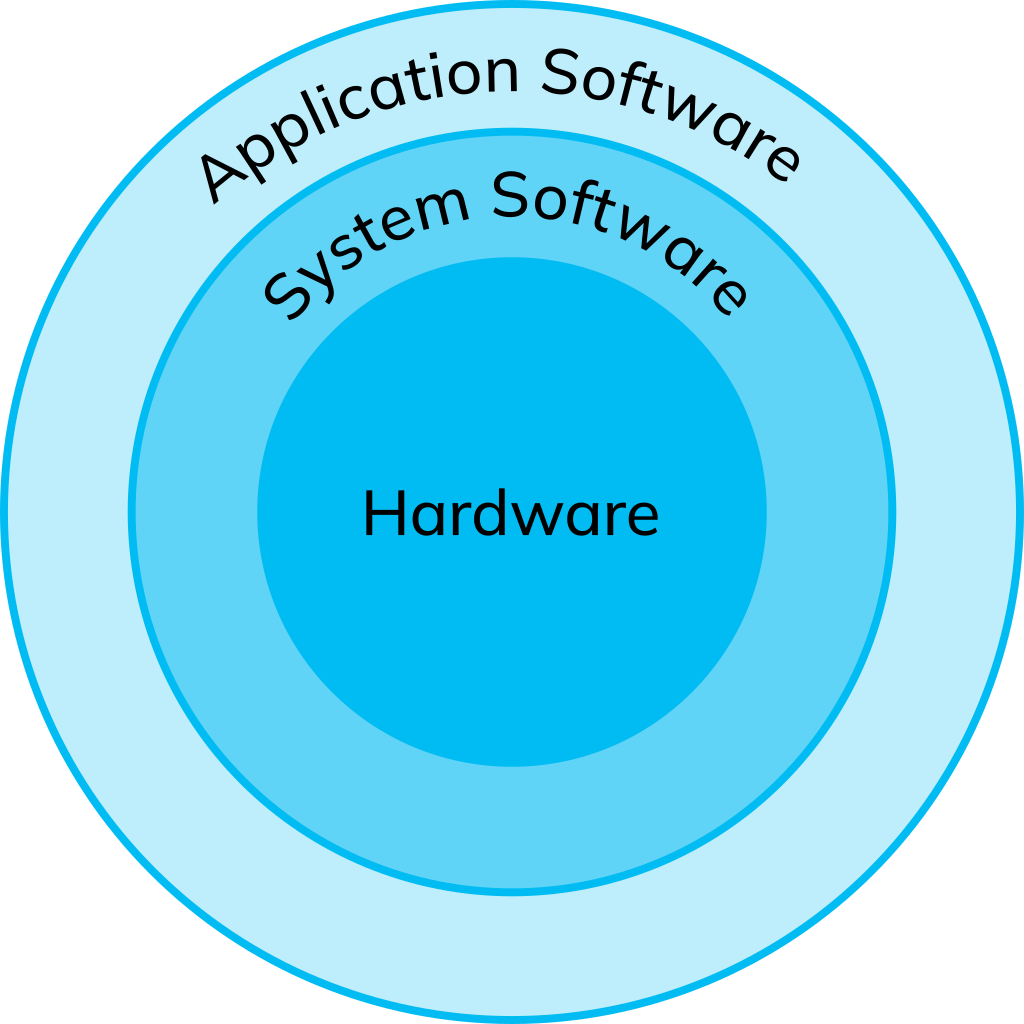
\includegraphics[width=\linewidth]{figures/Layers of SW.png}
\end{minipage}


\subsection{HW and SW}

Both hardware and soft ware consist of hierarchical layers, with each
lower layer hiding details from the level above. One key interface
between the levels of abstraction is the instruction set architecture—
the interface between the hardware and low-level soft ware.

\begin{figure}[H]
   \centering
   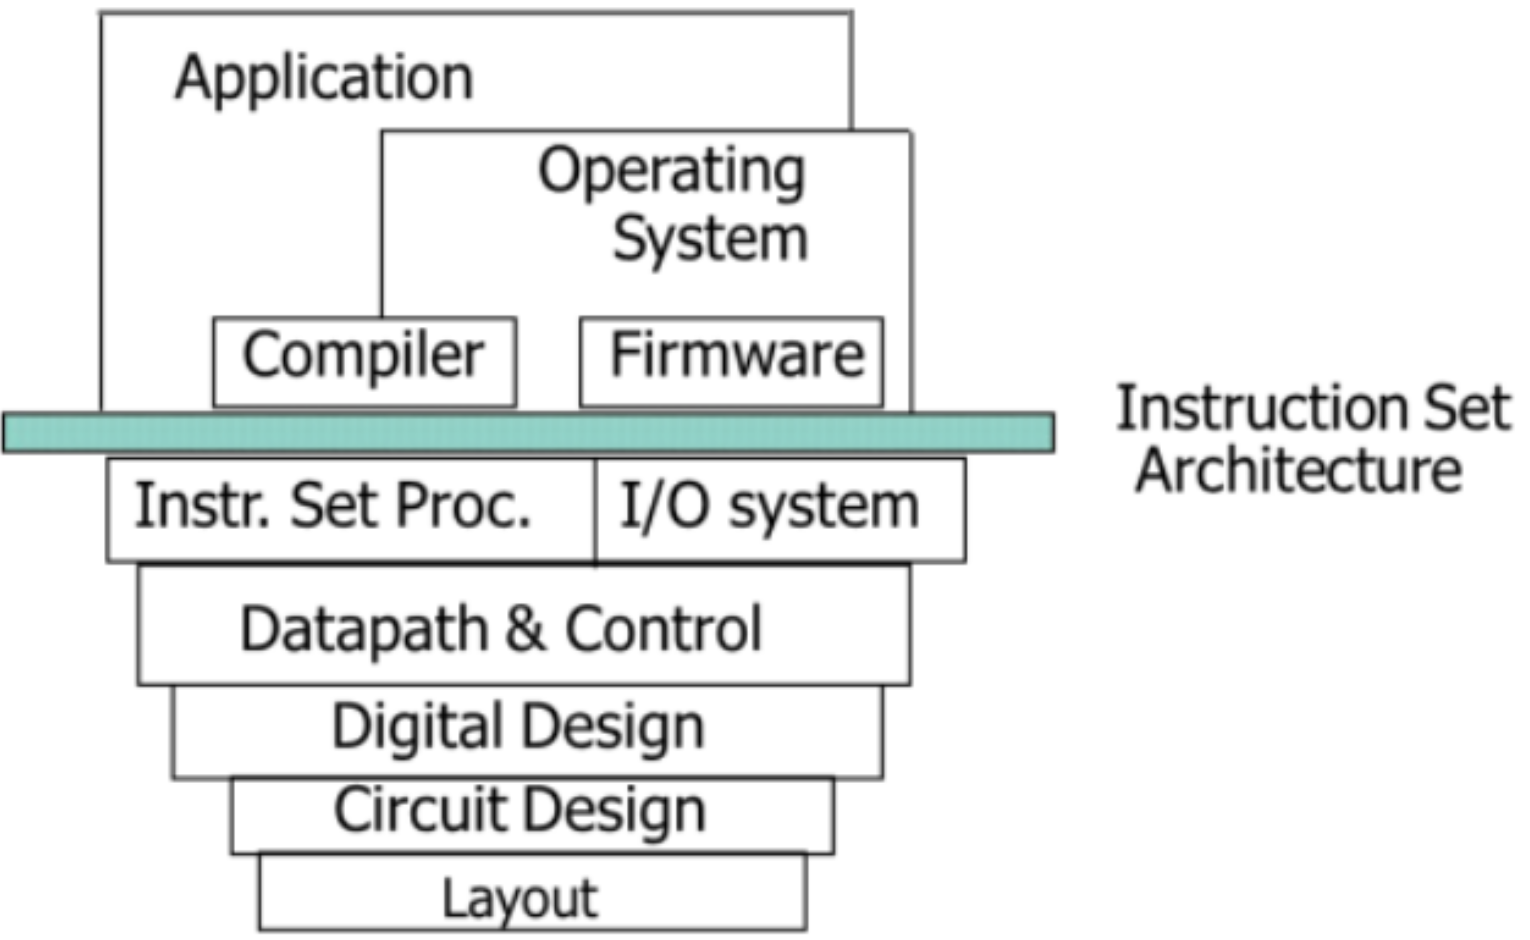
\includegraphics[width=0.4\linewidth]{figures/HwSw.png}
\end{figure}


% \section{Flynn's taxonomy}
% Flynn's taxonomy is a classification scheme for computer architectures proposed by Michael Flynn in 1966. The taxonomy is based on the number of instruction streams and data streams that can be processed simultaneously by a computer architecture.

% There are four categories in Flynn's taxonomy:\\
% \begin{minipage}[TH]{0.76\textwidth}
%    \textbf{Single Instruction Single Data (SIMD)}\\[0.5ex]
%    A uni-processor system that executes one instruction on one data stream at a time.

%    \begin{itemize}[parsep=0.5ex,left=0pt]
%       \item Instructions are processed in a \orange{sequential manner}, making SISD systems known as sequential computers.
%       \item Instructions and data are must be \orange{stored in primary memory}, and processing speed depends on internal data transfer rates.
%       \item \textbf{Examples}: Von Neumann Architecture, IBM PC and workstations.
%    \end{itemize}
% \end{minipage}\hfill
% \begin{minipage}[TH]{0.22\textwidth}
%       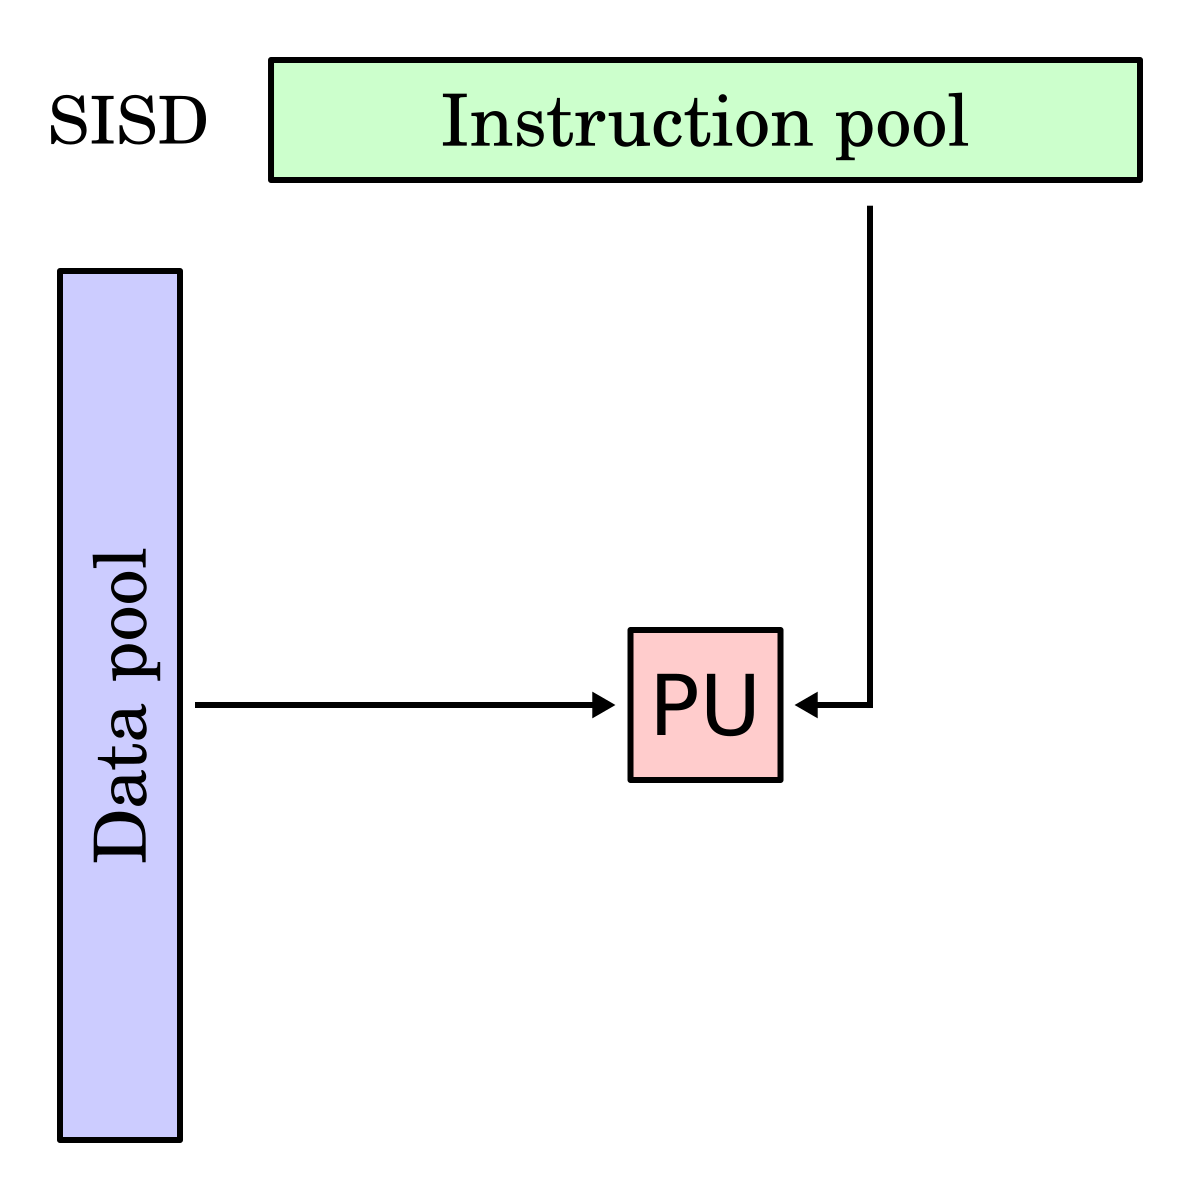
\includegraphics[width=\linewidth]{figures/sisd_diagram.png}
% \end{minipage}

% \begin{minipage}[TH]{0.76\textwidth}
%    \textbf{Single Instruction Multiple Data (SIMD)}\\[0.5ex]
%    A multiprocessor system where multiple processors execute the same instruction on different data streams.

%    \begin{itemize}[parsep=0.5ex,left=0pt]
%       \item Data elements are divided among multiple processing elements (PEs) for simultaneous computation.
%       \item Well-suited for vector and matrix operations.
%       \item \textbf{Examples}: Cray's vector processing machines.
%    \end{itemize}
% \end{minipage}\hfill
% \begin{minipage}[TH]{0.22\textwidth}
%       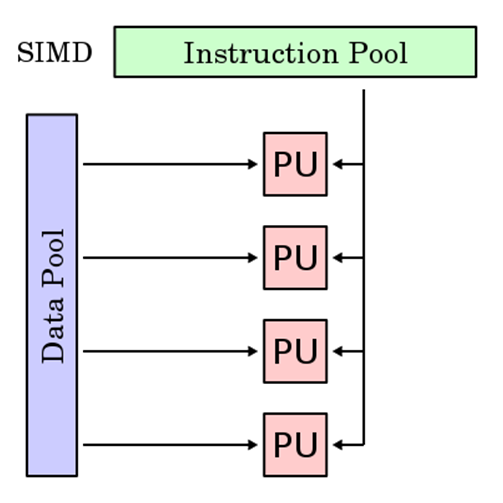
\includegraphics[width=\linewidth]{figures/simd_diagram.png}
% \end{minipage}

% \begin{minipage}[TH]{0.76\textwidth}
%    \textbf{Multiple Instruction Single Data (MISD)}\\[0.5ex]
%    A multiprocessor system where different processors execute different instructions on the same dataset.

%    \begin{itemize}[parsep=0.5ex,left=0pt]
%       \item Used in fault tolerance and error correction by applying different algorithms to the same data.
%       \item Not well-suited for typical computing needs, as most tasks require processing large data sets.
%       \item \textbf{Examples}: Rarely used in real-world applications.
%    \end{itemize}
% \end{minipage}\hfill
% \begin{minipage}[TH]{0.22\textwidth}
%       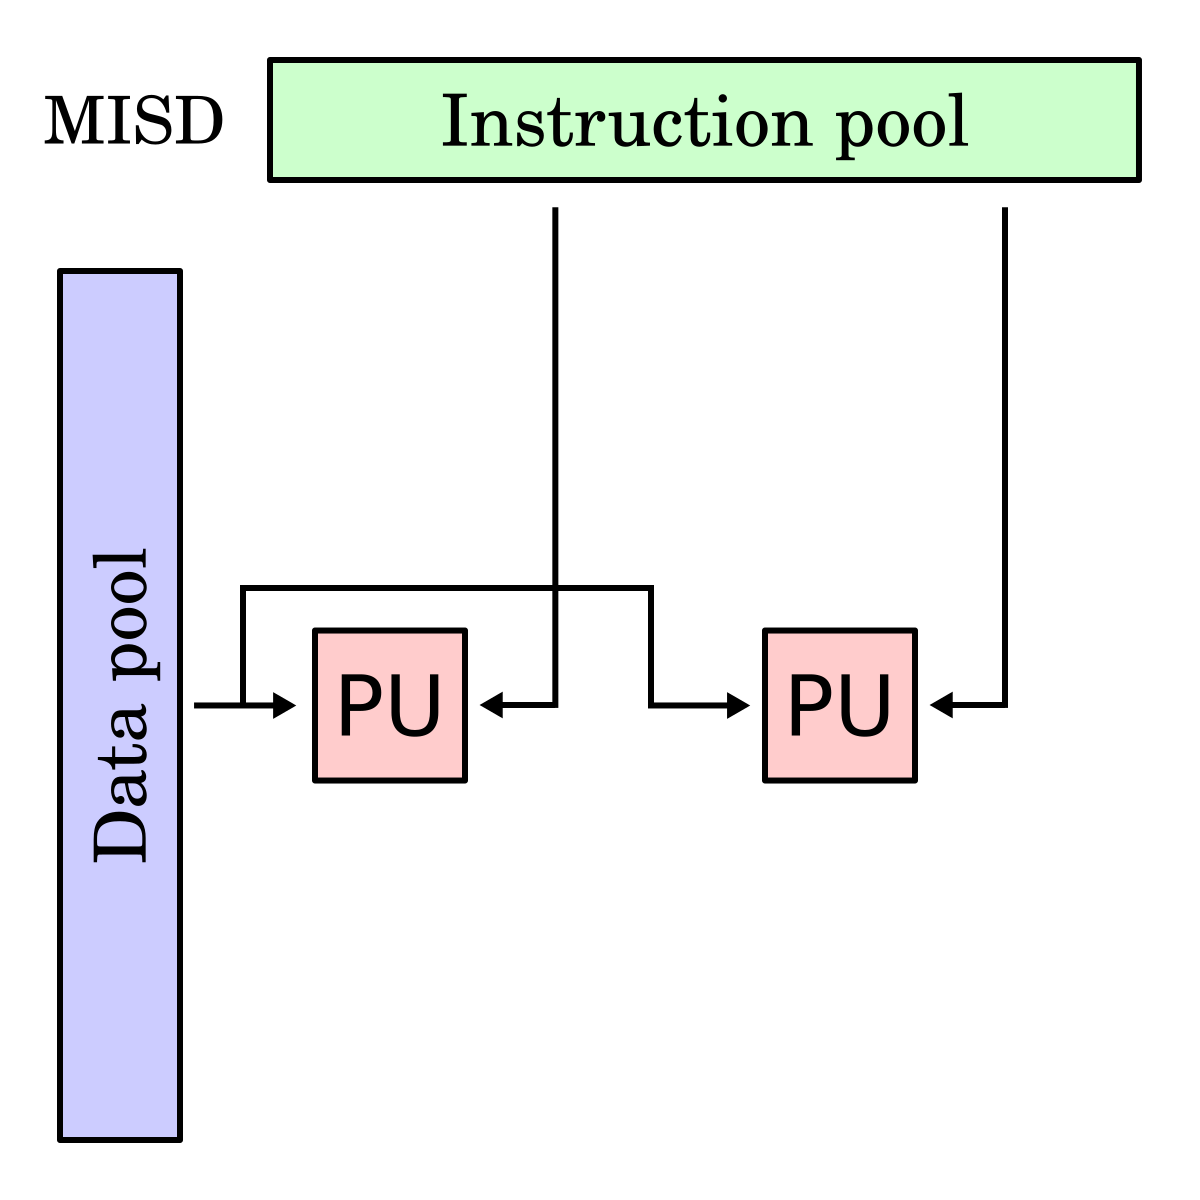
\includegraphics[width=\linewidth]{figures/misd_diagram.png}
% \end{minipage}

% \begin{minipage}[TH]{0.76\textwidth}
%    \textbf{Multiple Instruction Multiple Data (MIMD)}\\[0.5ex]
%    A multiprocessor system that executes multiple instructions on multiple data sets, with each processor having separate instruction and data streams.

%    \begin{itemize}[parsep=0.5ex,left=0pt]
%       \item PEs in MIMD machines work asynchronously, allowing flexibility for a wide range of applications.
%       \item Shared-Memory MIMD: All PEs share a single global memory, and communication occurs through this shared memory.
%       \item Distributed-Memory MIMD: All PEs are connected to local memory with no global memory access.
%       \item \textbf{Examples}: Multi-Core Processors, SMP systems, GPUs.
%    \end{itemize}
% \end{minipage}\hfill
% \begin{minipage}[TH]{0.22\textwidth}
%       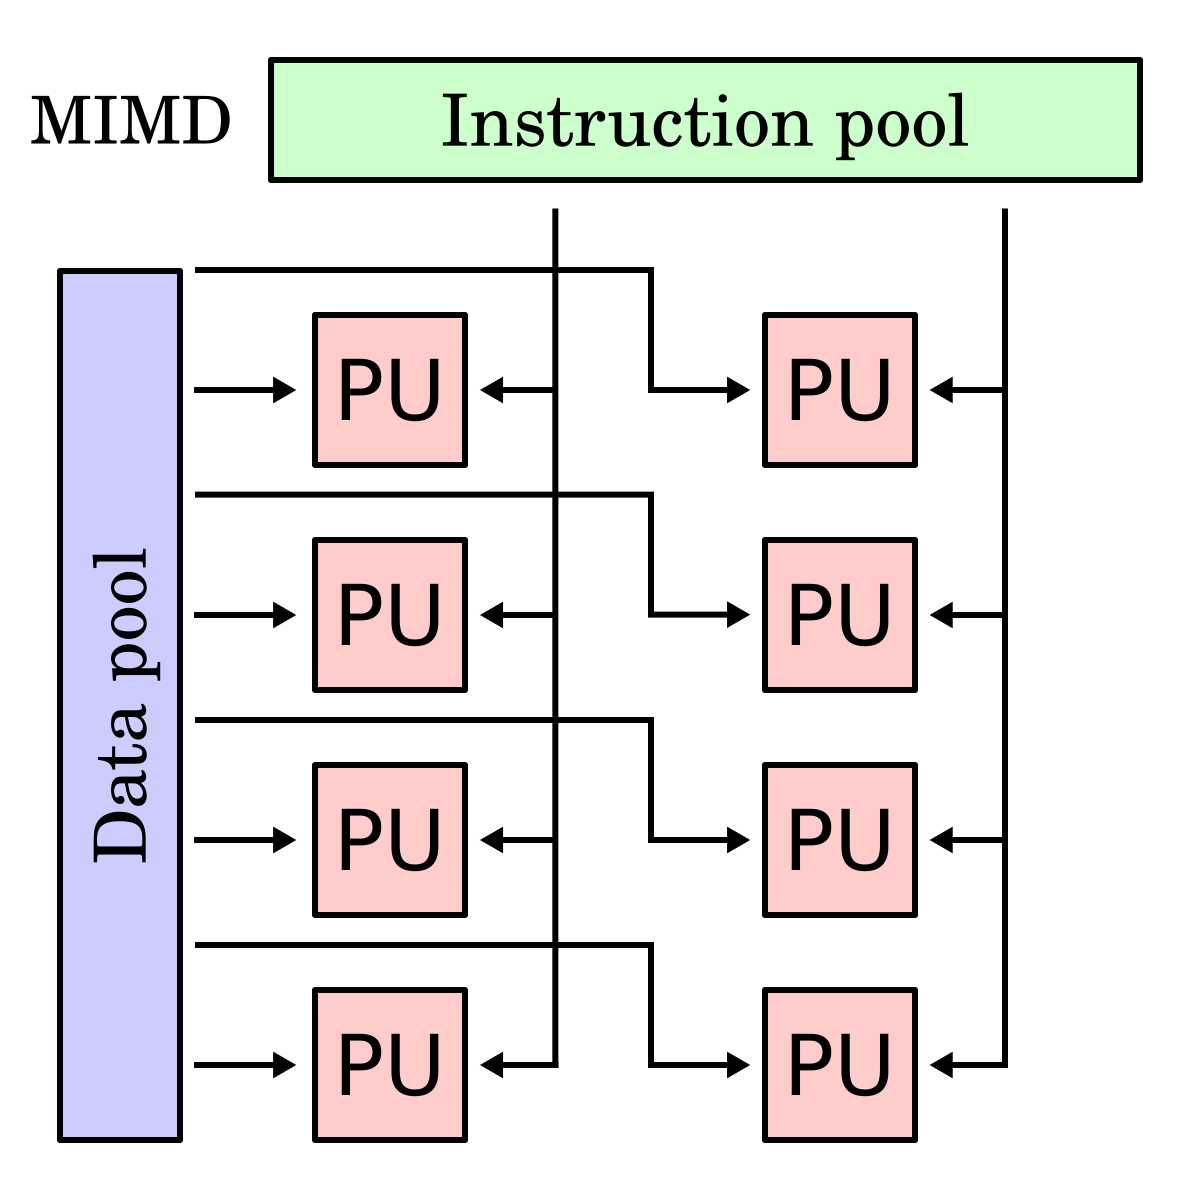
\includegraphics[width=\linewidth]{figures/mimd_diagram.png}
% \end{minipage}